\documentclass[11pt]{article}

% Use Helvetica font.
\usepackage{helvet}
\renewcommand{\familydefault}{\sfdefault}
\usepackage[utf8x]{inputenc}
\usepackage[margin=0.75in]{geometry}
\usepackage{graphicx}
\usepackage{wrapfig}

\usepackage{lipsum}
\usepackage{amssymb,amsfonts,amsmath}
\usepackage{bm}
\usepackage{url}
%\usepackage[table]{xcolor}
\usepackage{booktabs}
\usepackage{caption}
%\captionsetup{skip&=0pt}
\usepackage[numbers,sort&compress]{natbib}
\bibliographystyle{unsrtnat}
\setcitestyle{numbers,square,comma}
%\usepackage{cite}
\usepackage{enumitem}
%\usepackage{xcolor,colortbl}
%\bibliographystyle{nihunsrt} 
\usepackage{multicol}
\usepackage[dvipsnames, table]{xcolor}
\newcommand{\ddt}[1]{\frac{d#1}{dt}}

\begin{document}
%\section{Simple models of LAIV and IIV}
%\begin{multicols}{2}
%Model of LAIV:
%\begin{align}
%\begin{split}
%\ddt{L} &&= rL - kLX_q\\
%\ddt{X_G} &&= sX_G \frac{L}{\phi_{LG} + L}\\
%\ddt{X_S} &&= sX_S \frac{L}{\phi_{LS} + L}
%\end{split}
%\end{align}
%
%
%Model of IIV
%\begin{align}
%\begin{split}
%\ddt{I} &&= -rI - kIX_q\\
%\ddt{X_G} &&= sX_q \frac{I}{\phi_{IG} + I}\\
%\ddt{X_S} &&= sX_S \frac{I}{\phi_{IS} + I}
%\end{split}
%\end{align}
%\end{multicols}

\section{Mathematical model}
\begin{align}
\mbox{target cells}\quad    \ddt{T} &= -\beta TV\\
\mbox{infected cells}\quad    \ddt{I} &= \beta TV -k_RT_{R}I - \delta I\\
\mbox{viral titer}\quad    \ddt{V} &= pI - cV - f(A_O, V)*k_A V A_O - f(A_V, V)*k_A V A_V\\
%\mbox{free antigen}\quad    \ddt{H} &= \gamma V - d_H H - f(Ab, V)* k_A H Ab\\
\mbox{B-cells for old strain}\quad \ddt{B_O} &= g(A_O, V)*\frac{\sigma V }{\phi_{A} + V} \\
\mbox{antibodies for old strain}\quad    \ddt{A_0} &= \kappa B_0 - d_{A}A_O \\
\mbox{B-cells for vaccine strain}\quad \ddt{B_V} &= g(A_V, V)*\frac{\sigma V }{\phi_{A} + V} \\
\mbox{antibodies for vaccine strain}\quad    \ddt{A_V} &= \kappa B_V - d_{A}A_V\\
\mbox{expanding}\quad    \ddt{T_{E}} &= \rho T_{E}\Big(\frac{I}{\phi + I}\Big) - (\alpha + r)T_{E}\Big(1 - \frac{I}{\phi + I}\Big) - \mu T_{E}\\
\mbox{memory}\quad    \ddt{T_{M}} &= rT_{E}\Big(1 - \frac{I}{\phi+I}\Big)\\
\mbox{resident}\quad    \ddt{T_{R}} &= \mu  T_{E}   - d_R  T_{R}
\end{align}

where the parameter $f(Ab, V)$ is a multiplier modifying the antibody response as a function of antigenic-antibody distance. This function is  a Hill-type function, given by:

$$ f(x) = \frac{-M x^n}{K^n + x^n} + 1$$
$M$, $K$, and $n$ are parameters to be determined.
The variable $x$ measures the percentage of antigenic distance between antibodies $A$ and virus $V$. The antigenic distance can be given by any of the available distances (there are many antigenic distances out there, starting with the one proposed by Smith et al in 1999). I like to think about this as the  fraction of amino acid differences in the dominant epitope between the antibody and the virus (taken from Gupta et al, 2006). With this set of parameters, the function $f(x)$ looks like this:

\begin{figure}[htbp]
\begin{center}
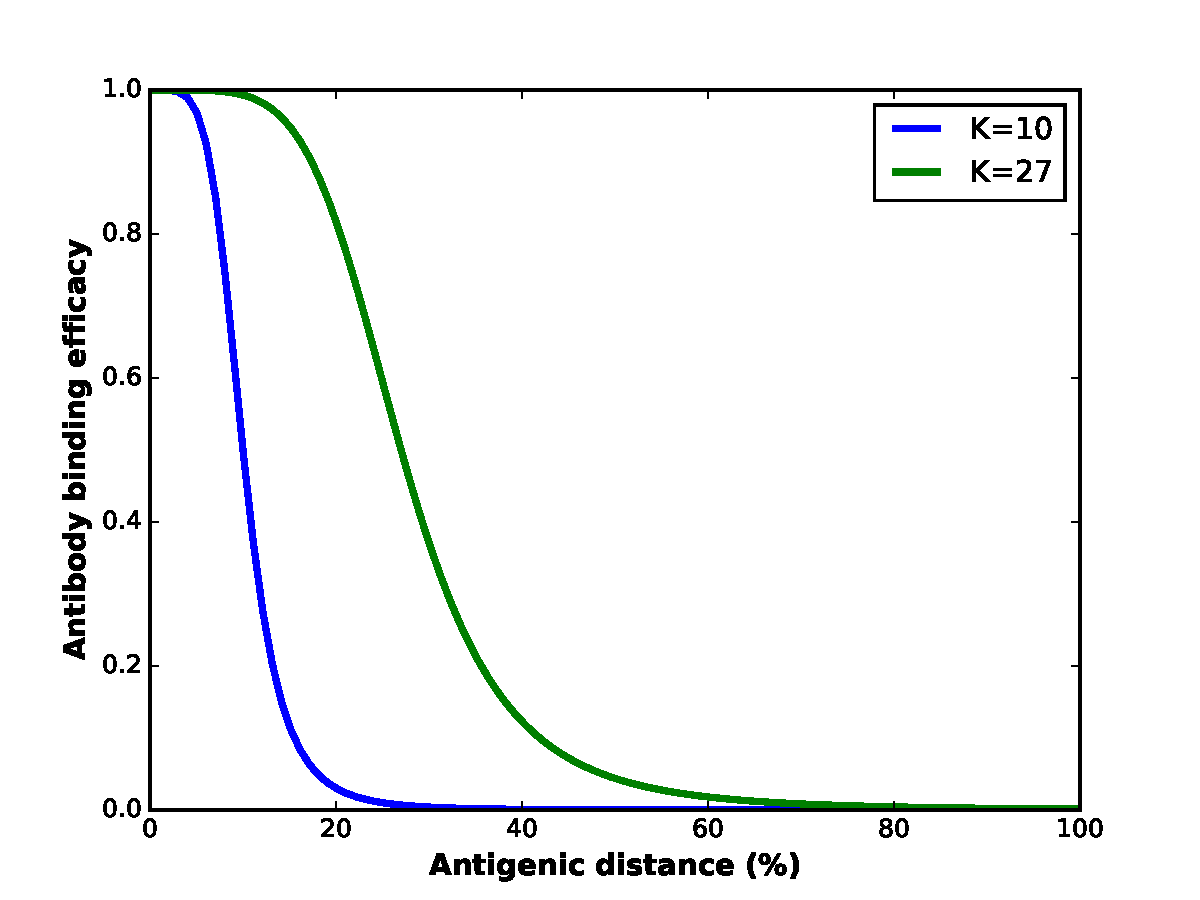
\includegraphics[scale=0.5]{functionAntigenicDistance.pdf}
\caption{Antibody efficacy as a function of antigenic distance for two different values of $K$.}
\label{figantigenicDistance}
\end{center}
\end{figure}

If $x=0$, it is a perfect match. The parameters were chosen so that once the distance reaches $~25\%$ (left panel) or $~75\%$ (right panel) , the antibody stops being  reactive to the antigen.
\\



\begin{table}[htp]
\caption{Model parameters defintions and values.}
\begin{center}
\begin{tabular}{lclcl}
\toprule
Model parameter & Symbol & Units & Value & Reference\\
\midrule
Rate of apoptosis for $T_E$ &$\alpha$ &&\\
Virus infectivity & $\beta$ &&\\
Rate of viral clearance & $c$ &&\\
Infected-cell lifespan & $1/\delta$ &&\\
Rate of antibody decay &$d_{A}$ &&\\
Death rate of $T_R$ & $d_R$ &&\\
Rate of antibody production & $\kappa$ $$\\
Rate of killing of virus by antigen & $k_A$ &&\\
Rate of killing of infected cells by $T_R$ & $k_R$ &&\\
Rate of conversion from $T_E$ to $T_R$ & $\mu$ &&\\
Virus production per cell & $p$ &&\\
Number of infected cells for half-max. proliferation &$\phi$ &&\\
Number of virus for half-max. B-cell activation &$\phi_{A}$ &&\\
Rate of conversion from $T_E$ to $T_M$ & $r$ &&\\
 T-cell proliferation rate &$\rho$ &&\\
Max. activation rate of B-cells &$\sigma$&&\\
\end{tabular}
\end{center}
\label{default}
\end{table}%

\end{document}